\documentclass{standalone}
\usepackage{pgfplots}
\pgfplotsset{compat=1.18}

\begin{document}
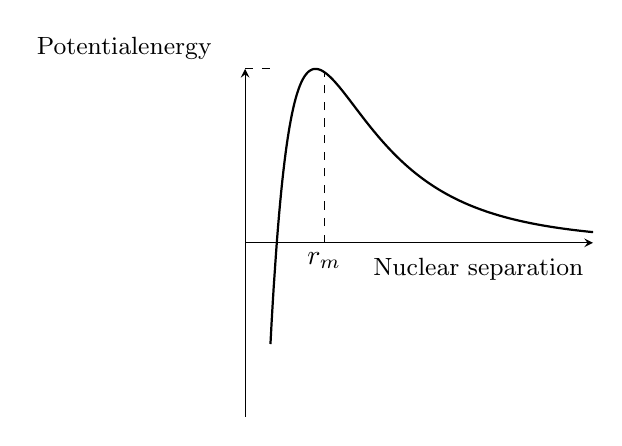
\begin{tikzpicture}
  \begin{axis}[
      axis lines=middle,
      xlabel={\small Nuclear separation},
      ylabel={\small Potential\\ energy},
      xtick=\empty,
      ytick=\empty,
      domain=0.9:2,
      samples=200,
      ymin=-1, ymax=1,
      xmin=0.9, xmax=2,
      width=6cm,
      height=6cm,
      %axis line style={->},
      every axis x label/.style={at={(current axis.right of origin)}, anchor=north east, yshift=-0.5ex},
      every axis y label/.style={at={(current axis.above origin)}, anchor=south east, xshift=-2ex},
      clip=false
  ]

    % Potential curve: a combination of repulsive (1/x^12) and attractive (1/x^6)
    \addplot[thick, domain=0.98:2, samples=300]
      {-4*((1/x)^12 - (1/x)^6)};

    % Equilibrium point r_m
    \draw[dashed] (axis cs:1.15, 0) -- (axis cs:1.15, 0.99);
    \node[below] at (axis cs:1.15, 0) {$r_m$};

    % Horizontal line showing e^2/(4π ε₀ r_m)
    \draw[dashed] (0.9, 1) -- (1, 1);
    %\node[left] at (0.9, 1) {$\dfrac{e^2}{4\pi \varepsilon_0 r_m}$};

  \end{axis}
\end{tikzpicture}
\end{document}
